\newcommand{\ee}{\mathrm{e}}
\newcommand{\ii}{\mathrm{i}}
\heading{数学物理方法（上）-第6次作业}

\begin{question}
计算下列积分：

1. \(\displaystyle f(z)=\oint_{|\zeta|=2} \frac{(\zeta^*)^2 \ee^{\zeta}}{\zeta-z} \dd{}\zeta\)，其中 \(\zeta^*\) 为复数 \(\zeta\) 的复共轭，\(z\) 为复数且 \(|z|\neq2\).

2. \(\displaystyle \oint_{|z|=1} \ln\frac{1+2z}{1-2z} \cdot \frac{dz}{z+2}\)，沿实轴从 \(\displaystyle -\frac12\) 到 \(\displaystyle \frac12\) 作割线，规定割线上岸 \(\displaystyle \arg\frac{1+2z}{1-2z}=2\pi\).

\begin{center}
\begin{tikzpicture}[scale=1.5]
\draw[->] (-2.5,0) -- (1.5,0) node[right] {$x$};
\draw[->] (0,-2) -- (0,2) node[above] {$y$};
\draw[blue,thick] (0,0) circle (1);
% Branch cut
\draw[red,thick] (-0.5,0.05) arc (90:270:0.05) -- (0.5,0.05) arc (90:-90:0.05);
\node at (0.5,-0.05) [below] {$\frac12$};
\node at (-0.5,-0.05) [below] {$-\frac12$};
\node at (-1,0) [below] {$-1$};
\node at (0,-1) [below] {$-i$};
\node at (0,1) [above] {$i$};
\node at (1,0) [above] {$1$};
\node at (-2,0) [above] {$-2$};
\end{tikzpicture}
\end{center}

\begin{solution}
(1) 在 \(|\zeta|=2\) 的圆上，\(\zeta^*=4/\zeta\)，代入可以得到
\[ f(z)=\oint_{|\zeta|=2} \frac{16\ee^{\zeta}}{\zeta^2(\zeta-z)}\dd{z} \]

考察 \(G(z,\eta)=\displaystyle\oint_{|\zeta|=2} \frac{16\ee^{\zeta}}{(\zeta-\eta)(\zeta-z)}\dd{}\zeta\)。由柯西积分公式可知，当 \(|z|>2,|\eta|<2\) 时，
\[ G(z,\eta)=2\pi\ii \cdot \frac{16\ee^{\eta}}{\eta-z} \]
因此有
\[ f(z)=\left.\dv{}{\eta}G(z,\eta)\right|_{\eta=0}=32\pi\ii \left.\frac{\ee^{\eta}(\eta-z)-\ee^{\eta}}{(\eta-z)^2}\right|_{\eta=0}=32\pi\ii\frac{-1-z}{z^2} \]

当 \(|z|<2,|\eta|<2\) 时，有
\[ G(z,\eta)=\oint_{|\zeta|=2}\frac{16\ee^{\zeta}}{\eta-z}\Bigl(\frac1{\zeta-\eta}-\frac1{\zeta-z}\Bigr)\dd{}\zeta=\frac{32\pi\ii(\ee^{\eta}-\ee^{z})}{\eta-z} \]
因此有
\[ f(z)=\left.\dv{}{\eta}G(z,\eta)\right|_{\eta=0}=\left.\frac{32\pi\ii\bigl(\ee^{\eta}(\eta-z)-(\ee^{\eta}-\ee^{z})\bigr)}{(\eta-z)^2}\right|_{\eta=0}=32\pi\ii\frac{\ee^{z}-z-1}{z^2} \]

综上有
\[ f(z)=\begin{cases}
32\pi\ii\cdot\dfrac{-z-1}{z^2}, & |z|>2,\\[6pt]
32\pi\ii\cdot\dfrac{\ee^{z}-z-1}{z^2}, & |z|<2
\end{cases} \]

(2) 在上述割线的定义下 \(f(z)=\ln\dfrac{1+2z}{1-2z}\) 在 \(\mathbb{C}\setminus\text{割线}\) 上解析。先考察一半径为 \(R\) 的大圆 \(C_R\) 与积分围道 \(C\) 组成的区域

\begin{center}
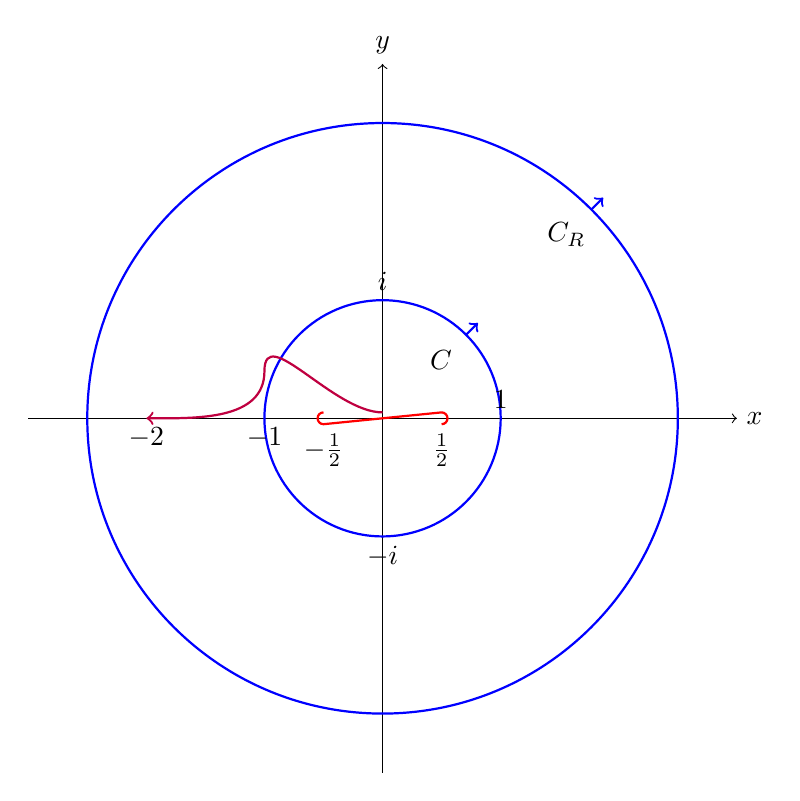
\begin{tikzpicture}[scale=1.5]
\draw[->] (-3,0) -- (3,0) node[right] {$x$};
\draw[->] (0,-3) -- (0,3) node[above] {$y$};
\draw[blue,thick] (0,0) circle (1);
\draw[blue,thick] (0,0) circle (2.5);
% Branch cut
\draw[red,thick] (-0.5,0.05) arc (90:270:0.05) -- (0.5,0.05) arc (90:-90:0.05);
% Labels
\node at (0.5,-0.05) [below] {$\frac12$};
\node at (-0.5,-0.05) [below] {$-\frac12$};
\node at (-1,0) [below] {$-1$};
\node at (0,-1) [below] {$-i$};
\node at (0,1) [above] {$i$};
\node at (1,0) [above] {$1$};
\node at (-2,0) [below] {$-2$};
\draw[->,blue,thick] (45:2.5) -- ++(0.1,0.1);
\draw[->,blue,thick] (45:1) -- ++(0.1,0.1);
\node at (45:2.2) {$C_R$};
\node at (45:0.7) {$C$};
% Purple path from 0 to -2
\draw[purple,thick,->] (0,0.05) to[out=180,in=90] (-1,0.4) to[out=-90,in=0] (-2,0);
\end{tikzpicture}
\end{center}

有
\[ \oint_{C_R} \frac{f(z)}{z+2}\dd{z} + \oint_{C} \frac{f(z)}{z+2}\dd{z} = 2\pi\ii f(-2) \]

因此我们只需要计算 \(\oint_{C_R} f(z)/(z+2)\dd{z}\) 与 \(f(-2)\) 即可。先计算 \(f(-2)\)，考察沿图中紫色路径改变输入 \(z\)，这一过程中
\[ \Delta\arg\frac{1+2z}{1-2z} = \Delta\arg\Bigl(z+\frac12\Bigr) - \Delta\arg\Bigl(z-\frac12\Bigr) = \pi \]
因此
\[ \left.\arg\frac{1+2z}{1-2z}\right|_{z=-2} = \left.\arg\frac{1+2z}{1-2z}\right|_{z=0} + \Delta\arg = 3\pi \]
\[ f(-2)=\ln\Bigl|\frac{1+2z}{1-2z}\Bigr| + \ii\arg\frac{1+2z}{1-2z} = \ln\frac35 + 3\pi\ii \]

接下来计算 \(\displaystyle\oint_{C_R} \frac{f(z)}{z+2}\dd{z}\)，注意到
\[ \lim_{z\to\infty} \frac{z\,f(z)}{z+2} = \lim_{z\to\infty} f(z)=3\pi\ii \]
极限存在，因此由大圆弧引理
\[ \oint_{C_R} \frac{f(z)}{z+2}\dd{z} = \ii\cdot 3\pi\ii\cdot (2\pi-0) = -6\pi^2 \]

故我们可以计算得到
\[ \oint_{C} \frac{f(z)}{z+2}\dd{z} = 2\pi\ii f(-2) - \oint_{C_R} \frac{f(z)}{z+2}\dd{z} = -6\pi^2 + 2\pi\ii\ln\frac35 + 6\pi^2 = 2\pi\ii\ln\frac35. \]

综上，我们可以得到
\[ \oint_{|z|=1} \frac{f(z)}{z+2}\dd{z} = -\oint_{C} \frac{f(z)}{z+2}\dd{z} = -2\pi\ii\ln\frac35. \]
\end{solution}
\end{question}

\begin{question}
计算下列积分：

1. \(\displaystyle \oint_{|z|=2} \frac{\sin z}{z^4}\dd{z}\);\qquad
2. \(\displaystyle \oint_{|z|=2} \frac{dz}{z^2(z^2+16)}\);\qquad
3. \(\displaystyle \oint_{|z|=2} \frac{|z|\ee^{z}}{z^2}\dd{z}\).

\begin{solution}

(1) 考察函数 \(f(z)=\displaystyle\oint_{|\xi|=2} \frac{\phi(\xi)}{\xi-z}\dd{}\xi\)，其中 \(\phi(\xi)=\sin\xi\) 在围道上连续。当 \(|z|<2\) 时，由柯西积分公式，可以得到
\[ f(z)=2\pi\ii\,\phi(z)=2\pi\ii\sin z \]
因此有
\[ f^{(3)}(z)=3! \oint_{|\xi|=2} \frac{\phi(\xi)}{(\xi-z)^4}\dd{}\xi = -2\pi\ii\cos z \]
代入 \(z=0\) 可以得到
\[ \oint_{|\xi|=2} \frac{\sin\xi}{\xi^4}\dd{}\xi = -\frac{\pi}{3}\ii. \]

(2) 考察函数 \(f(z)=\displaystyle\oint_{|\xi|=2} \frac{\phi(\xi)\dd{}\xi}{\xi-z}\)，其中 \(\phi(\xi)=\dfrac1{\xi^2+16}\) 在围道上连续。当 \(|z|<2\) 时，由柯西积分公式，可以得到
\[ f(z)=2\pi\ii\,\phi(z)=2\pi\ii\cdot\frac1{z^2+16} \]
因此有
\[ f'(z)=\oint_{|\xi|=2} \frac{\phi(\xi)}{(\xi-z)^2}\dd{}\xi = -\frac{2\pi\ii}{(z^2+16)^2}\cdot 2z \]
代入 \(z=0\) 可以得到
\[ \oint_{|\xi|=2} \frac{\phi(\xi)}{\xi^2}\dd{}\xi = 0. \]

(3) 考察函数 \(f(z)=\displaystyle\oint_{|\xi|=2} \frac{\phi(\xi)\dd{}\xi}{\xi-z}\)，其中 \(\phi(\xi)=2\ee^{z}\) 在围道上连续。当 \(|z|<2\) 时，由柯西积分公式，可以得到
\[ f(z)=2\pi\ii\,\phi(z)=2\pi\ii\cdot2\ee^{z} \]
因此有
\[ f'(z)=\oint_{|\xi|=2} \frac{\phi(\xi)}{(\xi-z)^2}\dd{}\xi = 4\pi\ii\,\ee^{z} \]
代入 \(z=0\) 可以得到
\[ \oint_{|\xi|=2} \frac{\phi(\xi)}{\xi^2}\dd{}\xi = 4\pi\ii. \]
\end{solution}
\end{question}

\begin{question}
1. 计算积分 \(\displaystyle \oint_{|z|=1} \frac{\ee^{z}}{z^3}\dd{z}\)；

2. \(a\) 取何值时，变上限积分 \(\displaystyle F(z)=\int_{z_0}^{z} \ee^{\zeta}\Bigl(\frac1\zeta+\frac{a}{\zeta^3}\Bigr)\dd{}\zeta\) 在 \(z\) 复平面内是单值的？

\begin{solution}
(1) 考察函数 \(f(z)=\displaystyle\oint_{|\xi|=1} \frac{\ee^{\xi}}{\xi-z}\dd{z}\)，因此有根据柯西积分公式，当 \(|z|<1\) 时
\[ f(z)=2\pi\ii\,\ee^{z} \]
因此由 \(\ee^{\xi}\) 在 \(|\xi|=1\) 曲线上的连续性，可以知道
\[ f^{(2)}(z)=2! \oint_{|\xi|=1} \frac{\ee^{\xi}}{(\xi-z)^3}\dd{}\xi = 2\pi\ii\,\ee^{z} \]
代入 \(z=0\)，可以得到
\[ \oint_{|\xi|=1} \frac{\ee^{\xi}}{\xi^3} = \pi\ii.  \]

(2) 注意到 \(f(\zeta)=\ee^{\zeta}\Bigl(\dfrac1\zeta+\dfrac{a}{\zeta^3}\Bigr)\) 在 \(\mathbb{C}\setminus\{0\}\) 上解析。故若我们考察从 \(z_0\) 到 \(z\) 的两条不同的积分路径 \(\gamma_1,\gamma_2\)，若 \(\gamma_1,\gamma_2\) 围出的区域不包含 \(0\)，则
\[ \int_{\gamma_1} f(\zeta)\dd{}\zeta-\int_{\gamma_2} f(\zeta)\dd{}\zeta = 0 \]
即积分值只取决于初末点。若 \(\gamma_1,\gamma_2\) 围出的区域包含 \(0\)，为了使 \(F(z)\) 是单值的，则要求
\[ \oint_C f(\zeta)\dd{}\zeta = 0 \]
其中 \(C\) 围出的区域包含 \(0\).

考察函数 \(G(z)=\displaystyle\oint_C \frac{\ee^{\xi}}{\xi-z}\dd{}\xi\)，根据柯西积分公式有 \(G(z)=2\pi\ii\,\ee^{z}\).

由于 \(\ee^{\xi}\) 在 \(C\) 上连续，因此
\[ G^{(2)}(z)=2! \oint_C \frac{\ee^{\xi}}{(\xi-z)^3}\dd{}\xi = 2\pi\ii\,\ee^{z} \]

代入 \(z
\end{question}
\end{solution}
